\documentclass[10pt]{article}
\usepackage[T1]{fontenc}

% Document Details
\newcommand{\CLASS}{AMATH 584}
\newcommand{\assigmentnum}{Assignment 2}

\usepackage[margin = 1.15in, top = 1.25in, bottom = 1.in]{geometry}

\usepackage{titling}
\setlength{\droptitle}{-6em}   % This is your set screw
\date{}
\renewcommand{\maketitle}{
	\clearpage
	\begingroup  
	\centering
	\LARGE \sffamily\textbf{\CLASS} \Large \assigmentnum\\[.8em]
	\large Tyler Chen\\[1em]
	\endgroup
	\thispagestyle{empty}
}
 % Title Styling
\usepackage{tocloft}
\renewcommand{\cfttoctitlefont}{\Large\sffamily\bfseries}
\renewcommand{\cftsecfont}{\normalfont\sffamily\bfseries}
\renewcommand{\cftsubsecfont}{\normalfont\sffamily}
\renewcommand{\cftsubsubsecfont}{\normalfont\sffamily}

\makeatletter
\let\oldl@section\l@section
\def\l@section#1#2{\oldl@section{#1}{\sffamily\bfseries#2}}

\let\oldl@subsection\l@subsection
\def\l@subsection#1#2{\oldl@subsection{#1}{\sffamily#2}}

\let\oldl@subsubsection\l@subsubsection
\def\l@subsubsection#1#2{\oldl@subsubsection{#1}{\sffamily#2}}
 % General Styling


\usepackage{enumitem}

% Figures
\usepackage{subcaption}

% TikZ and Graphics
\usepackage{tikz, pgfplots}
\pgfplotsset{compat=1.12}
\usetikzlibrary{patterns,arrows}
\usepgfplotslibrary{fillbetween}

\usepackage{pdfpages}
\usepackage{adjustbox}

\usepackage{lscape}
\usepackage{titling}
\usepackage[]{hyperref}


% Header Styling
\usepackage{fancyhdr}
\pagestyle{fancy}
\lhead{\sffamily \CLASS}
\rhead{\sffamily Chen \textbf{\thepage}}
\cfoot{}

% Paragraph Styling
\setlength{\columnsep}{1cm}
\setlength{\parindent}{0pt}
\setlength{\parskip}{5pt}
\renewcommand{\baselinestretch}{1}

% TOC Styling
\usepackage{tocloft}
\iffalse
\renewcommand{\cftsecleader}{\cftdotfill{\cftdotsep}}

\renewcommand\cftchapafterpnum{\vskip6pt}
\renewcommand\cftsecafterpnum{\vskip10pt}
\renewcommand\cftsubsecafterpnum{\vskip6pt}

% Adjust sectional unit title fonts in ToC
\renewcommand{\cftchapfont}{\sffamily}
\renewcommand{\cftsecfont}{\bfseries\sffamily}
\renewcommand{\cftsecnumwidth}{2em}
\renewcommand{\cftsubsecfont}{\sffamily}
\renewcommand{\cfttoctitlefont}{\hfill\bfseries\sffamily\MakeUppercase}
\renewcommand{\cftaftertoctitle}{\hfill}

\renewcommand{\cftchappagefont}{\sffamily}
\renewcommand{\cftsecpagefont}{\bfseries\sffamily}
\renewcommand{\cftsubsecpagefont}{\sffamily}
\fi
 % General Styling
% Code Display Setup
\usepackage{listings,lstautogobble}
\usepackage{lipsum}
\usepackage{courier}
\usepackage{catchfilebetweentags}

\lstset{
	basicstyle=\small\ttfamily,
	breaklines=true, 
	frame = single,
	rangeprefix=,
	rangesuffix=,
	includerangemarker=false,
	autogobble = true
}


\usepackage{algorithmicx}
\usepackage{algpseudocode}

\newcommand{\To}{\textbf{to}~}
\newcommand{\DownTo}{\textbf{downto}~}
\renewcommand{\algorithmicdo}{\hspace{-.2em}\textbf{:}}
 % Code Display Setup
% AMS MATH Styling
\usepackage{amsmath, amssymb}
\newcommand{\qed}{\hfill\(\square\)}

%\newtheorem*{lemma}{Lemma} 
%\newtheorem*{theorem}{Theorem}
%\newtheorem*{definition}{Definition}
%\newtheorem*{prop}{Proposition}
%\renewenvironment{proof}{{\bfseries Proof.}}{}


% mathcal
\newcommand{\cA}{\ensuremath{\mathcal{A}}}
\newcommand{\cB}{\ensuremath{\mathcal{B}}}
\newcommand{\cC}{\ensuremath{\mathcal{C}}}
\newcommand{\cD}{\ensuremath{\mathcal{D}}}
\newcommand{\cE}{\ensuremath{\mathcal{E}}}
\newcommand{\cF}{\ensuremath{\mathcal{F}}}
\newcommand{\cG}{\ensuremath{\mathcal{G}}}
\newcommand{\cH}{\ensuremath{\mathcal{H}}}
\newcommand{\cI}{\ensuremath{\mathcal{I}}}
\newcommand{\cJ}{\ensuremath{\mathcal{J}}}
\newcommand{\cK}{\ensuremath{\mathcal{K}}}
\newcommand{\cL}{\ensuremath{\mathcal{L}}}
\newcommand{\cM}{\ensuremath{\mathcal{M}}}
\newcommand{\cN}{\ensuremath{\mathcal{N}}}
\newcommand{\cO}{\ensuremath{\mathcal{O}}}
\newcommand{\cP}{\ensuremath{\mathcal{P}}}
\newcommand{\cQ}{\ensuremath{\mathcal{Q}}}
\newcommand{\cR}{\ensuremath{\mathcal{R}}}
\newcommand{\cS}{\ensuremath{\mathcal{S}}}
\newcommand{\cT}{\ensuremath{\mathcal{T}}}
\newcommand{\cU}{\ensuremath{\mathcal{U}}}
\newcommand{\cV}{\ensuremath{\mathcal{V}}}
\newcommand{\cW}{\ensuremath{\mathcal{W}}}
\newcommand{\cX}{\ensuremath{\mathcal{X}}}
\newcommand{\cY}{\ensuremath{\mathcal{Y}}}
\newcommand{\cZ}{\ensuremath{\mathcal{Z}}}

% mathbb
\usepackage{bbm}
\newcommand{\bOne}{\ensuremath{\mathbbm{1}}}

\newcommand{\bA}{\ensuremath{\mathbb{A}}}
\newcommand{\bB}{\ensuremath{\mathbb{B}}}
\newcommand{\bC}{\ensuremath{\mathbb{C}}}
\newcommand{\bD}{\ensuremath{\mathbb{D}}}
\newcommand{\bE}{\ensuremath{\mathbb{E}}}
\newcommand{\bF}{\ensuremath{\mathbb{F}}}
\newcommand{\bG}{\ensuremath{\mathbb{G}}}
\newcommand{\bH}{\ensuremath{\mathbb{H}}}
\newcommand{\bI}{\ensuremath{\mathbb{I}}}
\newcommand{\bJ}{\ensuremath{\mathbb{J}}}
\newcommand{\bK}{\ensuremath{\mathbb{K}}}
\newcommand{\bL}{\ensuremath{\mathbb{L}}}
\newcommand{\bM}{\ensuremath{\mathbb{M}}}
\newcommand{\bN}{\ensuremath{\mathbb{N}}}
\newcommand{\bO}{\ensuremath{\mathbb{O}}}
\newcommand{\bP}{\ensuremath{\mathbb{P}}}
\newcommand{\bQ}{\ensuremath{\mathbb{Q}}}
\newcommand{\bR}{\ensuremath{\mathbb{R}}}
\newcommand{\bS}{\ensuremath{\mathbb{S}}}
\newcommand{\bT}{\ensuremath{\mathbb{T}}}
\newcommand{\bU}{\ensuremath{\mathbb{U}}}
\newcommand{\bV}{\ensuremath{\mathbb{V}}}
\newcommand{\bW}{\ensuremath{\mathbb{W}}}
\newcommand{\bX}{\ensuremath{\mathbb{X}}}
\newcommand{\bY}{\ensuremath{\mathbb{Y}}}
\newcommand{\bZ}{\ensuremath{\mathbb{Z}}}

% alternative mathbb
\newcommand{\NN}{\ensuremath{\mathbb{N}}}
\newcommand{\RR}{\ensuremath{\mathbb{R}}}
\newcommand{\CC}{\ensuremath{\mathbb{C}}}
\newcommand{\ZZ}{\ensuremath{\mathbb{Z}}}
\newcommand{\EE}{\ensuremath{\mathbb{E}}}
\newcommand{\PP}{\ensuremath{\mathbb{P}}}
\newcommand{\VV}{\ensuremath{\mathbb{V}}}
\newcommand{\cov}{\ensuremath{\text{Co}\VV}}
% Math Commands

\newcommand{\st}{~\big|~}
\newcommand{\stt}{\text{ st. }}
\newcommand{\ift}{\text{ if }}
\newcommand{\thent}{\text{ then }}
\newcommand{\owt}{\text{ otherwise }}

\newcommand{\norm}[1]{\left\lVert#1\right\rVert}
\newcommand{\snorm}[1]{\lVert#1\rVert}
\newcommand{\ip}[1]{\ensuremath{\left\langle #1 \right\rangle}}
\newcommand{\pp}[3][]{\frac{\partial^{#1}#2}{\partial #3^{#1}}}
\newcommand{\dd}[3][]{\frac{\d^{#1}#2}{\d #3^{#1}}}
\renewcommand{\d}{\ensuremath{\mathrm{d}}}

\newcommand{\indep}{\rotatebox[origin=c]{90}{$\models$}}




 % Math shortcuts
% Problem
\usepackage{floatrow}

\newenvironment{problem}[1][]
{\pagebreak
\noindent\rule{\textwidth}{1pt}\vspace{0.25em}
{\sffamily \textbf{#1}}
\par
}
{\par\vspace{-0.5em}\noindent\rule{\textwidth}{1pt}}

\newenvironment{solution}[1][]
{{\sffamily \textbf{#1}}
\par
}
{}

 % Problem Environment

\newcommand{\note}[1]{\textcolor{red}{\textbf{Note:} #1}}

% overwrite old problem class to be able to add to ToC
\let\savedprob=\problem%
\def\problem[#1]{\pagebreak\phantomsection\addcontentsline{toc}{subsection}{#1}\savedprob[#1]\label{#1}}

\hypersetup{
   colorlinks=true,       % false: boxed links; true: colored links
   linkcolor=violet,          % color of internal links (change box color with linkbordercolor)
   citecolor=green,        % color of links to bibliography
   filecolor=magenta,      % color of file links
   urlcolor=cyan           % color of external links
}


\begin{document}
\maketitle

\begin{problem}[Exercise 3.5]
Example 3.6 shows that if \( E \) is an outer product \( E=uv^* \), then \( \norm{E}_2=\norm{u}_2\norm{v}_2 \). Is the same true for the Frobenius norm, i.e. \( \norm{E}_F = \norm{u}_F \norm{v}_F \)? Prove it or give a counterexample.
\end{problem}

\begin{solution}[Solution]
    Let \( E=uv^* \) for some \( u\in \RR^m \) and \( v\in \RR^n \). Denote the \( i \)-th component of \( v \) by \( v_i \).
We can then write \( E=[\overline{v_1}u, ..., \overline{v_n}u] \).

Observe that the Frobenius norm of a column vector is the 2-norm. Moreover, recall that the sum of the squares of the two norm of the columns of a matrix is equal to the square of the Frobenius norm of that matrix.

Thus,
\[ \norm{E}_F^2 = \sum_{i=1}^{n}\norm{\overline{v_i}u}_2^2 = \sum_{i=1}^{n}|\overline{v_i}|^2 \norm{u}_2^2 = \norm{u}_2^2 \sum_{i=1}^{n}|\overline{v_i}|^2 = \norm{u}_2^2 \sum_{i=1}^{n}|v_i|^2  =\norm{u}_2^2 \norm{v}_2^2 = \norm{u}_F^2 \norm{v}_F^2  \]


This proves that \( \norm{E}_F = \norm{u}_F \norm{v}_F \) for \( E=uv^* \). \qed

\end{solution}

\begin{problem}[Exercise 4.1]
    Determine the SVDs of the following matrices:
\begin{align*}
    \text{(a)} \left[\begin{array}{cc}3 & 0\\0 & -2\end{array}\right], && \text{(b)} \left[\begin{array}{cc}2 & 0\\0 & 3\end{array}\right] && \text{(c)} \left[\begin{array}{cc}0 & 2\\0 & 0\\0 & 0\end{array}\right], && \text{(d)} \left[\begin{array}{cc}1 & 1\\0 & 0\end{array}\right], && \text{(e)} \left[\begin{array}{cc}1 & 1 \\1 & 1\end{array}\right]
\end{align*}
\end{problem}

\begin{solution}[Solution]
Note that if \( A \) can be written \( A=U\Sigma V^* \) for \( U,V \) unitary, \( \Sigma \) real diagonal, then this is a SVD decomposition of \( A \). That is, we can simply attempt to manipulate \( A \) into a form which looks like the SVD and we will have found the SVD.

\begin{enumerate}
    \item[(a)]Here we simply have to switch the sign of the 2. We do this by right multiplying by a matrix which switches the sign of the second column and left multiplying by the identity.
        \begin{align*}
            \left[\begin{array}{cc}1 & 0\\0 & 1\end{array}\right]\left[\begin{array}{cc}3 & 0\\0 & 2\end{array}\right] \left[\begin{array}{cc}1 & 0 \\ 0 & -1\end{array}\right]
        \end{align*}
    \item[(b)]Here we need to switch the 2 and 3 so that the singular values are decreasing along the main diagonal. We switch the first and second columns and the first and second rows. 
         \begin{align*}
             \left[\begin{array}{cc}0 & 1\\1 & 0\end{array}\right]\left[\begin{array}{cc}3 & 0\\0 & 2\end{array}\right] \left[\begin{array}{cc}0 & 1\\1 & 0\end{array}\right]
        \end{align*}
    \item[(c)]Here we simply switch the first and second columns. 
        \begin{align*}
            \left[\begin{array}{ccc}1 & 0 & 0\\0 & 1 & 0\\0 & 0 & 1\end{array}\right] \left[\begin{array}{cc}2 & 0\\0 & 0\\0 & 0\end{array}\right] \left[\begin{array}{cc}0 & 1\\1 & 0\end{array}\right]
        \end{align*}
    \item[(d)]We observe this matrix is a rank 1 outer product \( xy^* \) of \( x=[1;0] \), \( y=[1,1] \). Therefore it has 2-norm equal to \( \norm{x}_2 \norm{y}_2 = 1\sqrt{2} = 2 \). Therefore, the first signular value is \( \sigma_1 = \sqrt{2} \). But as this matrix is rank 1, it has only 1 nonzero singular value. 
        
        We have \( Av_1 = \sigma u_1 \), for unit vectors \( u_1,v_1 \). Thus \( [v_{11}+v_{12} ; 0] = \sqrt{2}[u_{11} ; u_{12}] \) so \( u_{12} = 0 \). Since \( \norm{u_{1}}_2 = 1 \), WLOG let \( u_{11}=1 \). We also have \( v_{11}+v_{12}=\sqrt{2} \) and \( v_{11}^2+v_{12}^2=1 \). Together these give \( v_{11}=v_{12}=1/\sqrt{2} \).
        
        Since \( U \) is unitary, WLOG let \( u_{21}=0 \) and \( u_{22} = 1 \). Similarly, we require \( v_{11}^2+v_{21}^2 = 1 \) so, \( |v_{21}| = 1/\sqrt{2} \). Likewise, \( v_{12}^2+v_{22}^2=1 \) so, \( |v_{22}|=\sqrt{2} \). We also have \( Av_2 = [v_{21}+v_{22},0] = 0u_2 = 0 \). So \( v_{21}=-v_{22} \). Finally, we see that the sign has no impact. Therefore, we write,
        \begin{align*}
            \left[\begin{array}{cc}1 & 0\\0 & 1\end{array}\right]\left[\begin{array}{cc}\sqrt{2} & 0\\0 & 0\end{array}\right] \left[\begin{array}{cc}1/\sqrt{2} & 1/\sqrt{2}\\1/\sqrt{2} & -1/\sqrt{2}\end{array}\right]
        \end{align*}
    \item[(e)]We observe this matrix is a rank 1 outer product \( xy^* \) of \( x=[1;1] \), \( y=[1,1] \). Therefore it has 2-norm equal to \( \norm{x}_2 \norm{y}_2 = \sqrt{2}\sqrt{2} = 2 \). Therefore, the first singular value is \( 2 \). But as this matrix is rank 1, it has only 1 nonzero singular value.
        
        We have \( Av_1 = \sigma u_1 \), for unit vectors \( u_1,v_1 \). Thus \( [v_{11}+v_{12} ; v_{11}+v_{12}] = 2[u_{11} ; u_{12}] \) so \( u_{11} = u_{12} \). Since \( \norm{u_{1}}_2 = 1 \), then WLOG let \( u_{11}=u_{12} = 1/\sqrt{2} \). Therefore, \( v_{11}=v_{12}=1/\sqrt{2} \).
        
        We require \( v_{11}^2+v_{21}^2 = 1 \) so, \( |v_{21}| = 1/\sqrt{2} \). Likewise, \( v_{12}^2+v_{22}^2=1 \) so, \( |v_{22}|=\sqrt{2} \). We also have \( Av_2 = [v_{21}+v_{22},v_{21}+v_{22}] = 0u_2 = 0 \). So \( v_{21}=-v_{22} \). The sign has no impact so WLOG pick \( v_{21}=-v_{22}=1/\sqrt{2} \). Finally, by the same argument, note \( u_{21}=-u_{22} \) with \( |u_{21}|=|u_{22}|=1/\sqrt{2} \). However, in this case we require \( u_{21}=-u_{22} = 1/\sqrt{2} \).  Therefore, we write,

        \begin{align*}
           \left[\begin{array}{cc}1/\sqrt{2} & 1/\sqrt{2}\\1/\sqrt{2} & -1/\sqrt{2}\end{array}\right]\left[\begin{array}{cc}2 & 0\\0 & 0\end{array}\right] \left[\begin{array}{cc}1/\sqrt{2} & 1/\sqrt{2}\\1/\sqrt{2} & -1/\sqrt{2}\end{array}\right]
        \end{align*}
\end{enumerate}

%\textbf{IS THERE A BETTER WAY TO DO THIS???????? THIS PROBLEM IS ANNOYING AND NOT ENLIGHTENING} 
\end{solution}

\begin{problem}[Exercise 4.5]
Theorem 4.1 asserts that every \( A\in \CC^{m\times n} \) has an SVD \( A=U\Sigma V^* \). Show that if \( A \) is real, then it has a real SVD (\( U\in \RR^{m\times m}, V\in \RR^{n\times n} \)).
\end{problem}

\begin{solution}[Solution]
We first prove the following: \textit{If \( A\in\RR^{m\times m} \) has real eigenvalue \( \lambda \), then there exists a real unit eigenvector corresponding to \( \lambda \).}

Indeed, suppose \( v\in\CC^m \) is an eigenvector corresponding to \( \lambda \). That is, \( Av=\lambda v \). We can decompose \( v \) into its real and imaginary parts, \( x \) and \( y \) so that \( v=x+iy \). Then,
\begin{align*}
    \lambda x + i\lambda y = \lambda(x+iy) = \lambda v  Av = A(x_iy) = Ax+iAy
\end{align*}
Since \( \lambda \) is real, then \( \lambda x, \lambda y \) are real. Similarly, since \( A \) is real, then \( Ax, Ay \) are real. We can then equate real and imaginary parts to give, 
\begin{align*}
   Ax = \lambda x && Ay=\lambda y 
\end{align*}

Since \( w \) is an eigenvector of \( A \), \( w \) must be nonzero. This means at least one of \( x \) and \( y \) is nonzero. This vector is a real eigenvector of \( A \). Clearly we can scale this vector to obtain a real unit eigenvector. \qed

Next prove the following: \textit{If \( A\in\RR^{m\times m} \) is symmetric then there is an eigendecompsition \( AV=V\Lambda \), for \( \Lambda \) real and \( V \) unitary.}

Recall that for a Hermetian matrix all eigenvalues are real, and eigenvectors corresponding to distinct eigenvalues are orthogonal. Suppose \( \lambda \) is an eigenvalue with multiplicity \( k \). Then the eigenvectors corresponding to \( \lambda  \) form a \( k \)-dimensional subspace. But all vectors in this space are orthogonal to eigenvectors outside this space. Thus, by choosing an orthogonal basis for this set, we have \( k \) eigenvectors orthogonal to all other eigenvectors of \( A \).

This proves we can construct a basis for \( \CC^{m} \) of orthogonal eigenvectors for \( A \). Clearly these can be normalized. Let \( V \) be a matrix with the columns being the real, normal, orthogonal, eigenvectors of \( A \). Then \( V \) is real and unitary. Let \( \Lambda \) be a diagonal matrix with the eigenvalues corresponding to the eigenvectors in \( V \) placed on the diagonal. Then \( AV = V\Lambda \). \qed

If we order the eigenvalues of \( A \) in decreasing order, then \( AV=V\Lambda \) is unique up to scalar multiplication and rotation of any of the basis vectors of the subspaces corresponding to repeat eigenvalues.

Let \( A\in\RR^{m\times n} \). 

Suppose \( v \) is a unit eigenvalue of \( A^*A \). Then, \[ \lambda = \lambda v^*v = v^*\lambda v = v^*(A^*A)v=(v^*A^*)(Av) = (Av)^*(Av) = \norm{Av} \geq 0  \] 
This proves the eigenvalues of \( A^*A \) are positive.

We have \( A^*A \) is real Hermetian, so by the above results we have decomposition \( A^*AV=V\Lambda \) for some unitary \( V\in\RR^{n\times n} \). Moreover, we can reorder \( V \) and \( \Lambda \) such that the entries of \( \Lambda \) are decreasing in magnitude.


For convenience denote \( r \) as the number of nonzero entries of \( \Lambda \). That is \( r=\operatorname{rank}(A^*A) \).

We have \( r\leq \operatorname{min}(m,n) \) by rank arguments.

Define \( \Sigma\in\RR^{m\times n} \) by taking the square roots of the first \( r \) entries of \( \Lambda \) along the main diagonal. Leave all other entries zero.

For \( j\leq r \), \( \sigma_j\neq0 \), so define \( u_j:= Av_j/\sigma_j \). This gives a set \( \{ u_1, ..., u_r\} \) of real orthonormal vectors. Complete this set to a real orthonormal basis \( \{ \{u_1, ...., u_{r},u_{r+1}, ..., u_{m} \) of \( \RR^{m} \).

Then observe that for all \( j \), \( Av_j = \sigma_ju_j \). That is, \( AV=U\Sigma \) for \( V\in\RR^{n\times n}, U\in\RR^{m\times m} \) unitary, and \( \Sigma\in\RR^{m\times n} \) diagonal with positive decreasing entries.

That is, \( A=U\Sigma V^* \) is a real SVD for \( A \). \qed
\end{solution}
\begin{problem}[Exercise 5.4]
    Suppose \( A\in\CC^{m\times m} \) has an SVD \( A=U\Sigma V^* \). Find an eigenvalue decomposition of the \( 2m\times 2m \) Hermetian matrix
    \[ \left[\begin{array}{cc}0 & A^* \\ A & 0\end{array}\right] \]
\end{problem}

\begin{solution}[Solution]
Write the SVD of \( A \) as \( A=U\Sigma V^* \) so \( A^* = V\Sigma^*U^* = V\Sigma U^* \). Recall, for all \( 1\leq j\leq m, Av_j = \sigma_ju_j \) and \( A^*u_j=\sigma_jv_j \)

Then,
\begin{align*}
    \left[\begin{array}{cc}0 & A^* \\ A & 0\end{array}\right] \left[\begin{array}{c}v_j \\ u_j\end{array}\right] = \left[\begin{array}{c}A^*u_j \\ Av_j\end{array}\right] = \left[\begin{array}{c}\sigma_jv_j \\ \sigma_j u_j\end{array}\right] = \sigma_j \left[\begin{array}{c}v_j \\ u_j\end{array}\right]
\end{align*}
and similarly,
\begin{align*}
    \left[\begin{array}{cc}0 & A^* \\ A & 0\end{array}\right] \left[\begin{array}{c}v_j \\ -u_j\end{array}\right] = \left[\begin{array}{c}-A^*u_j \\ Av_j\end{array}\right] = \left[\begin{array}{c}-\sigma_jv_j \\ \sigma_j u_j\end{array}\right] = -\sigma_j \left[\begin{array}{c}v_j \\ -u_j\end{array}\right]
\end{align*}

That is, \( \left[\begin{array}{c}v_j\\u_j\end{array}\right] \) and \( \left[\begin{array}{c}v_j\\-u_j\end{array}\right] \) are eignevalues of \( \left[\begin{array}{cc}0 & A^*\\A & 0\end{array}\right] \) with corresponding eigenvalues \( \sigma_j \) and \( -\sigma_j \).

We can therefore write,
\begin{align*}
    \left[\begin{array}{cc}0 & A^*\\A & 0\end{array}\right] \left[\begin{array}{cc}V & V\\U & -U\end{array}\right] = 
        \left[\begin{array}{cc}V & V\\U & -U\end{array}\right] \left[\begin{array}{cc}\Sigma & 0\\0 & -\Sigma\end{array}\right]
\end{align*}


Therefore the above decomposition is close to the and eigen decomposition. However, observe,
\begin{align*}
    \left[\begin{array}{cc}V & V \\ U & -U\end{array}\right] \left[\begin{array}{cc}V & V \\ U & -U\end{array}\right]^* 
    &=  \left[\begin{array}{cc}V & V \\ U & -U\end{array}\right] \left[\begin{array}{cc}V^* & U^* \\ V^* & -U^*\end{array}\right] \\
    &= \left[\begin{array}{cc}VV^*+VV^* & VU^*-VU^*\\UV^*-UV^* & UU^*+UU^*\end{array}\right] \\
    &= \left[\begin{array}{cc}2I_m & 0 \\ 0 & 2I_m\end{array}\right] \\
    &= 2I_{2m}
\end{align*}

Therefore, define,
\begin{align*}
    X= \dfrac{1}{\sqrt{2}} \left[\begin{array}{cc} V & V \\ U & -U\end{array}\right] && \Lambda = \left[\begin{array}{cc}\Sigma & 0\\0 & \Sigma\end{array}\right]
\end{align*}

Then \( XX^* = I \), so the columns of \( X \) are orthonormal (and therefore lienarly independent) and  \( \Lambda \) is diagonal. Therefore, we have eigen decomposition,
\[ \left[\begin{array}{cc}0 & A^*\\A & 0\end{array}\right] = \left( \dfrac{1}{\sqrt{2}}\left[\begin{array}{cc} V & V \\ U & -U\end{array}\right]\right) \left[\begin{array}{cc}\Sigma & 0\\0 & -\Sigma\end{array}\right]\left( \dfrac{1}{\sqrt{2}}\left[\begin{array}{cc} V & V \\ U & -U\end{array}\right]\right)^* = X\Lambda X^* \tag*{\qed} \]
\end{solution}

\begin{problem}[Exercise (Image Compression)]
In Matlab, type {\tt imagedemo}.  You will see a picture of an Albrecht Durer print.  Type {\tt who} to see what variables it has used and type {\tt type imagedem} to see the actual Matlab code
that you have run.  You will see at the end that it executes the commands: \\
{\tt
imagesc(X); \\
colormap(map); \\
axis off;
} \\
The 648 by 509 matrix {\tt X} contains a grayscale number (from 1 to 128) for each pixel in a grid.
This number determines how dark or light that pixel will be shaded when the command 
{\tt imagesc(X)} is executed.  This is fine if one can store a 648 by 509 matrix, but if there are 
many such images and they are, say, being sent from outer space, using this large a matrix to represent 
each one could be prohibitive! \\
Compute the SVD of {\tt X}.  Try executing the above commands with {\tt X} replaced by some low rank
approximations formed from the largest singular values and corresponding singular vectors,
and decide about how many singular values/vectors are needed to make the picture recognizable.  
Turn in a few plots showing how the picture improves as you increase the rank
of the approximation used.  Label each plot with the rank of the approximation used.
[You can put several plots on one page using the {\tt subplot} command.
Type {\tt help subplot} to see exactly how it works.  You can save your plots to a file by
typing {\tt print -depsc hw2plots.eps} where the filename {\tt hw2plots} can be replaced
    by any name you like.]
\end{problem}

\begin{solution}[Solution]
    We first export the image matrix \verb|X| from MATLAB as a file \verb|img.mat|.

We then import with SciPy. We plot the original image. We compute the SVD of the matrix. We plot the rank-\( k \) approximation of the matrix for the listed \( k \). Note that rather than computing the rank-\( k \) approximation from \verb|X| we simply multiply the appropriate submatrices of \( U,V,S:=\Sigma \).

The outputs are saved and appended.

What it means for an image to be ``recognizable'' is vague, however the rank-50 approximation is pretty close to the original image, and the rank-150 image is almost indistinguishable from the original.

\lstinputlisting{hw2.py}

\begin{figure}[H]
    \centering
     \begin{subfigure}{.32\textwidth}
        \centering
        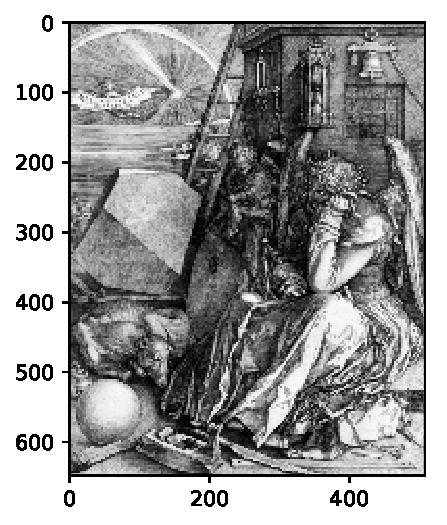
\includegraphics[width=.85\textwidth]{img/original.pdf}
        \caption{original}
    \end{subfigure}%
    \foreach \t in {509,300,150,100,50,30,20,10,5,1,0}{
    \begin{subfigure}{.32\textwidth}
        \centering
        \includegraphics[width=.85\textwidth]{img/\t.pdf}
        \caption{\( k=\t \)}
    \end{subfigure}%
    }
\end{figure}
\end{solution}


\end{document}
